\documentclass{article}

\title{The Best Place to \textit{Eat} and \textit{Drink} in the \textsc{Surfer's Paradise}}
\author{\textbf{A}ayush Baja\textbf{j}}
\usepackage{fancyhdr}
\usepackage[top=40mm,bottom=40mm,right=40mm,left=40mm]{geometry}

\usepackage{tcolorbox}
\usepackage{multicol}
\tcbuselibrary{theorems}
%\newtcbtheorem{mytheo}{@1}{colback=purple!5,colframe=blue!100!,fonttitle=\bfseries}{th}

\providecommand\theoremnumber{}
\newtcbtheorem{Theorembase}{Theorem \theoremnumber}{colback=purple!5,colframe=blue!100!,fonttitle=\bfseries}{Th}
\newenvironment{Theorem}[1]
 {\renewcommand{\theoremnumber}{#1}\begin{Theorembase*}}
 {\end{Theorembase*}}

\newtcbtheorem{Proofbase}{Proof \theoremnumber}{colback=purple!5,colframe=red!85!,fonttitle=\bfseries}{Th}
\newenvironment{Proof}[1]
 {\renewcommand{\theoremnumber}{#1}\begin{Proofbase*}}
 {\end{Proofbase*}}

\newtcbtheorem{Lemmabase}{Lemma \theoremnumber}{colback=purple!5,colframe=green!70!,fonttitle=\bfseries}{Th}
\newenvironment{Lemma}[1]
 {\renewcommand{\theoremnumber}{#1}\begin{Lemmabase*}}
 {\end{Lemmabase*}}

%unsw theorem
%\usepackage[tikz]{mdframed}
%\usepackage{xcolor,comment}
%\newmdenv[backgroundcolor=answerboxcolor]{answerbox}
%\colorlet{answerboxcolor}{blue!20}

\pagestyle{fancy}
\fancyhf{}
\fancyfoot[RO]{
    
\includegraphics[width=2cm]{qr.png}
}

\begin{document}
\maketitle
\thispagestyle{fancy}
\dotfill


\begin{Theorem}{1}{}
    Alfresco Italian Restaurant is the best place to eat and drink in the \textsc{Surfer's Paradise}.
\end{Theorem}

\begin{Lemma}{1}{}
    Let $P$ be the set of restaurants with affordable pricing, $E$ be the set of restaurants with high quality food, $N$ be the set of restaurants with good atmosphere, $I$ be the set of restaurants with good drinks and $S$ be the set of all restaurants with interesting culture.

    Then any $u \in U$ such that $u \in {P \cup E \cup N \cup I \cup S}$, where $U$ denotes the Universal set is a candidate for being "the best place to eat and drink in the \textsc{Surfer's Paradise}". 
\end{Lemma}

\begin{Proof}{1}{}
    Let $a$ be an arbitrary element in the universal set $U$, We must show that $a \in {P\cup E\cup N\cup I\cup S}$.

    \begin{multicols}{5}
        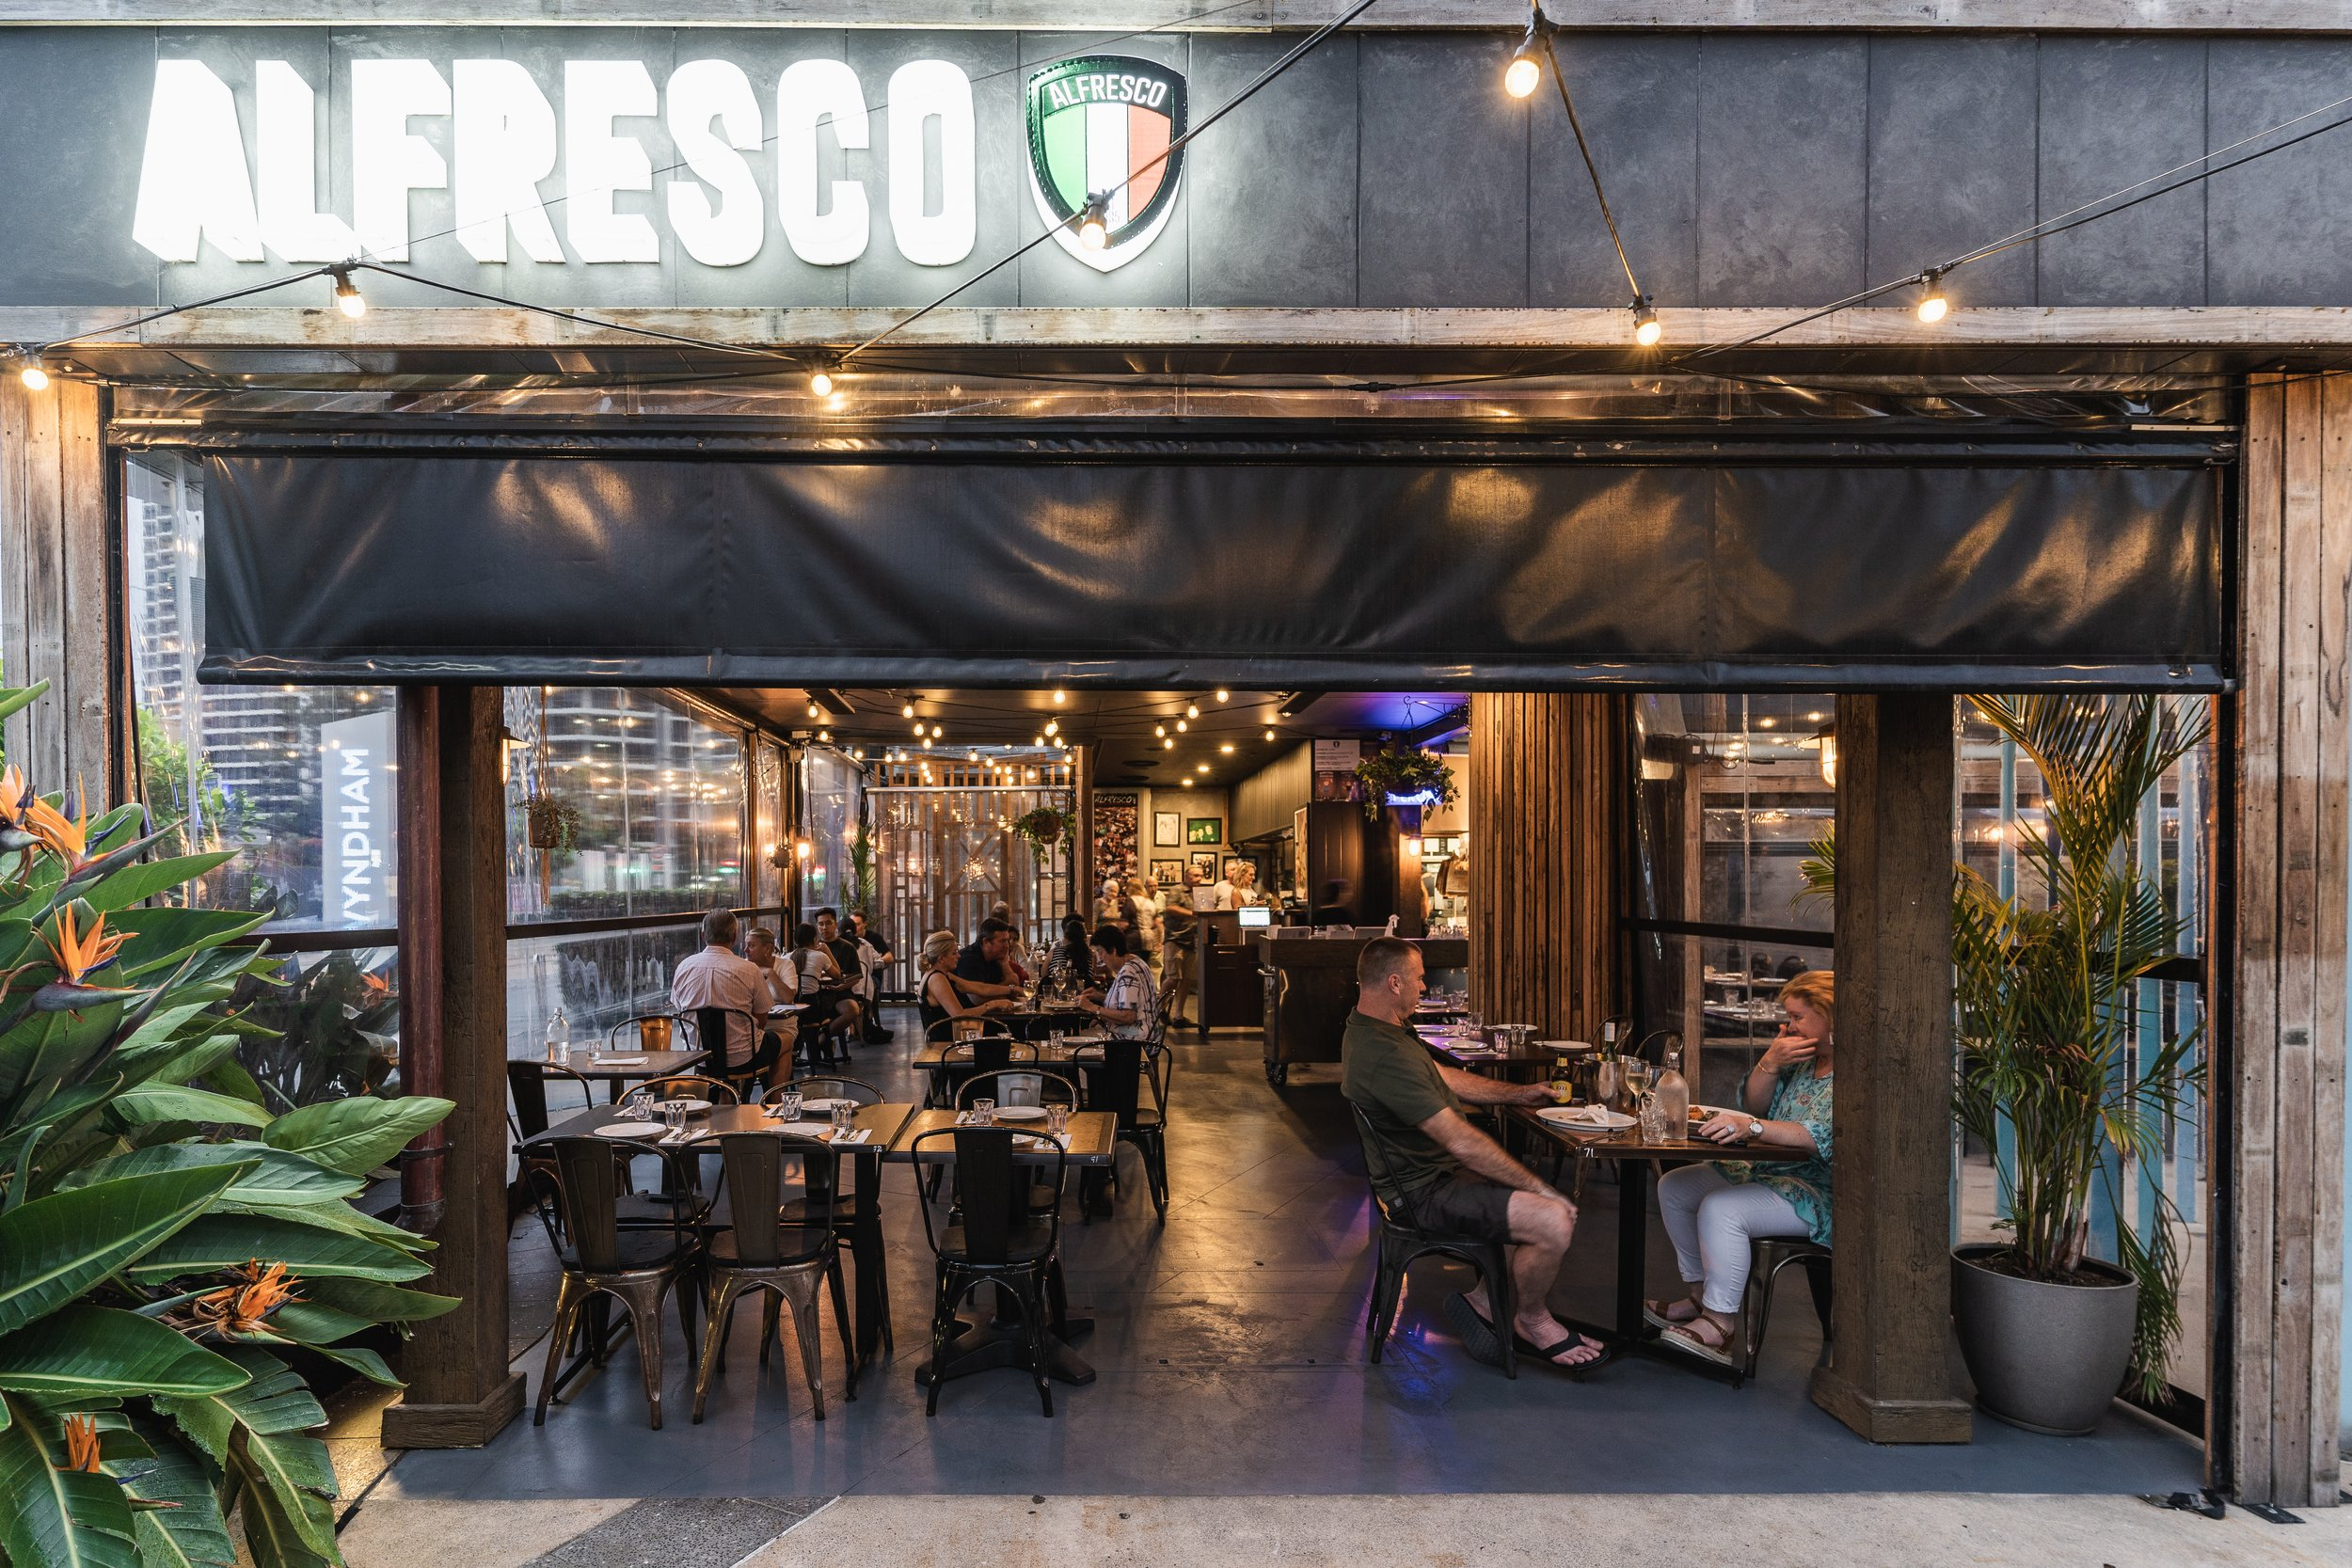
\includegraphics[width=3cm]{1.png}
        \hspace{1cm}
        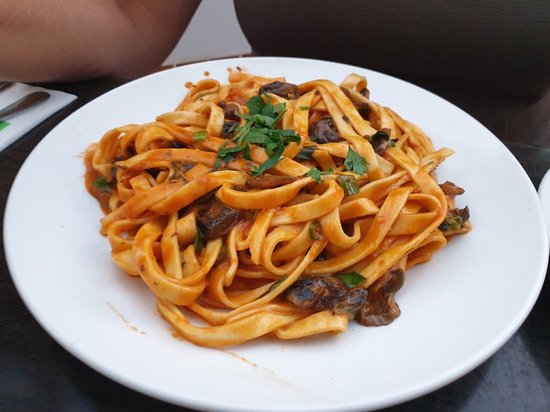
\includegraphics[width=2cm]{2.png}
        
\includegraphics[width=3cm]{3.png}
        
\includegraphics[width=3cm]{4.png}
        \hspace{1cm}
        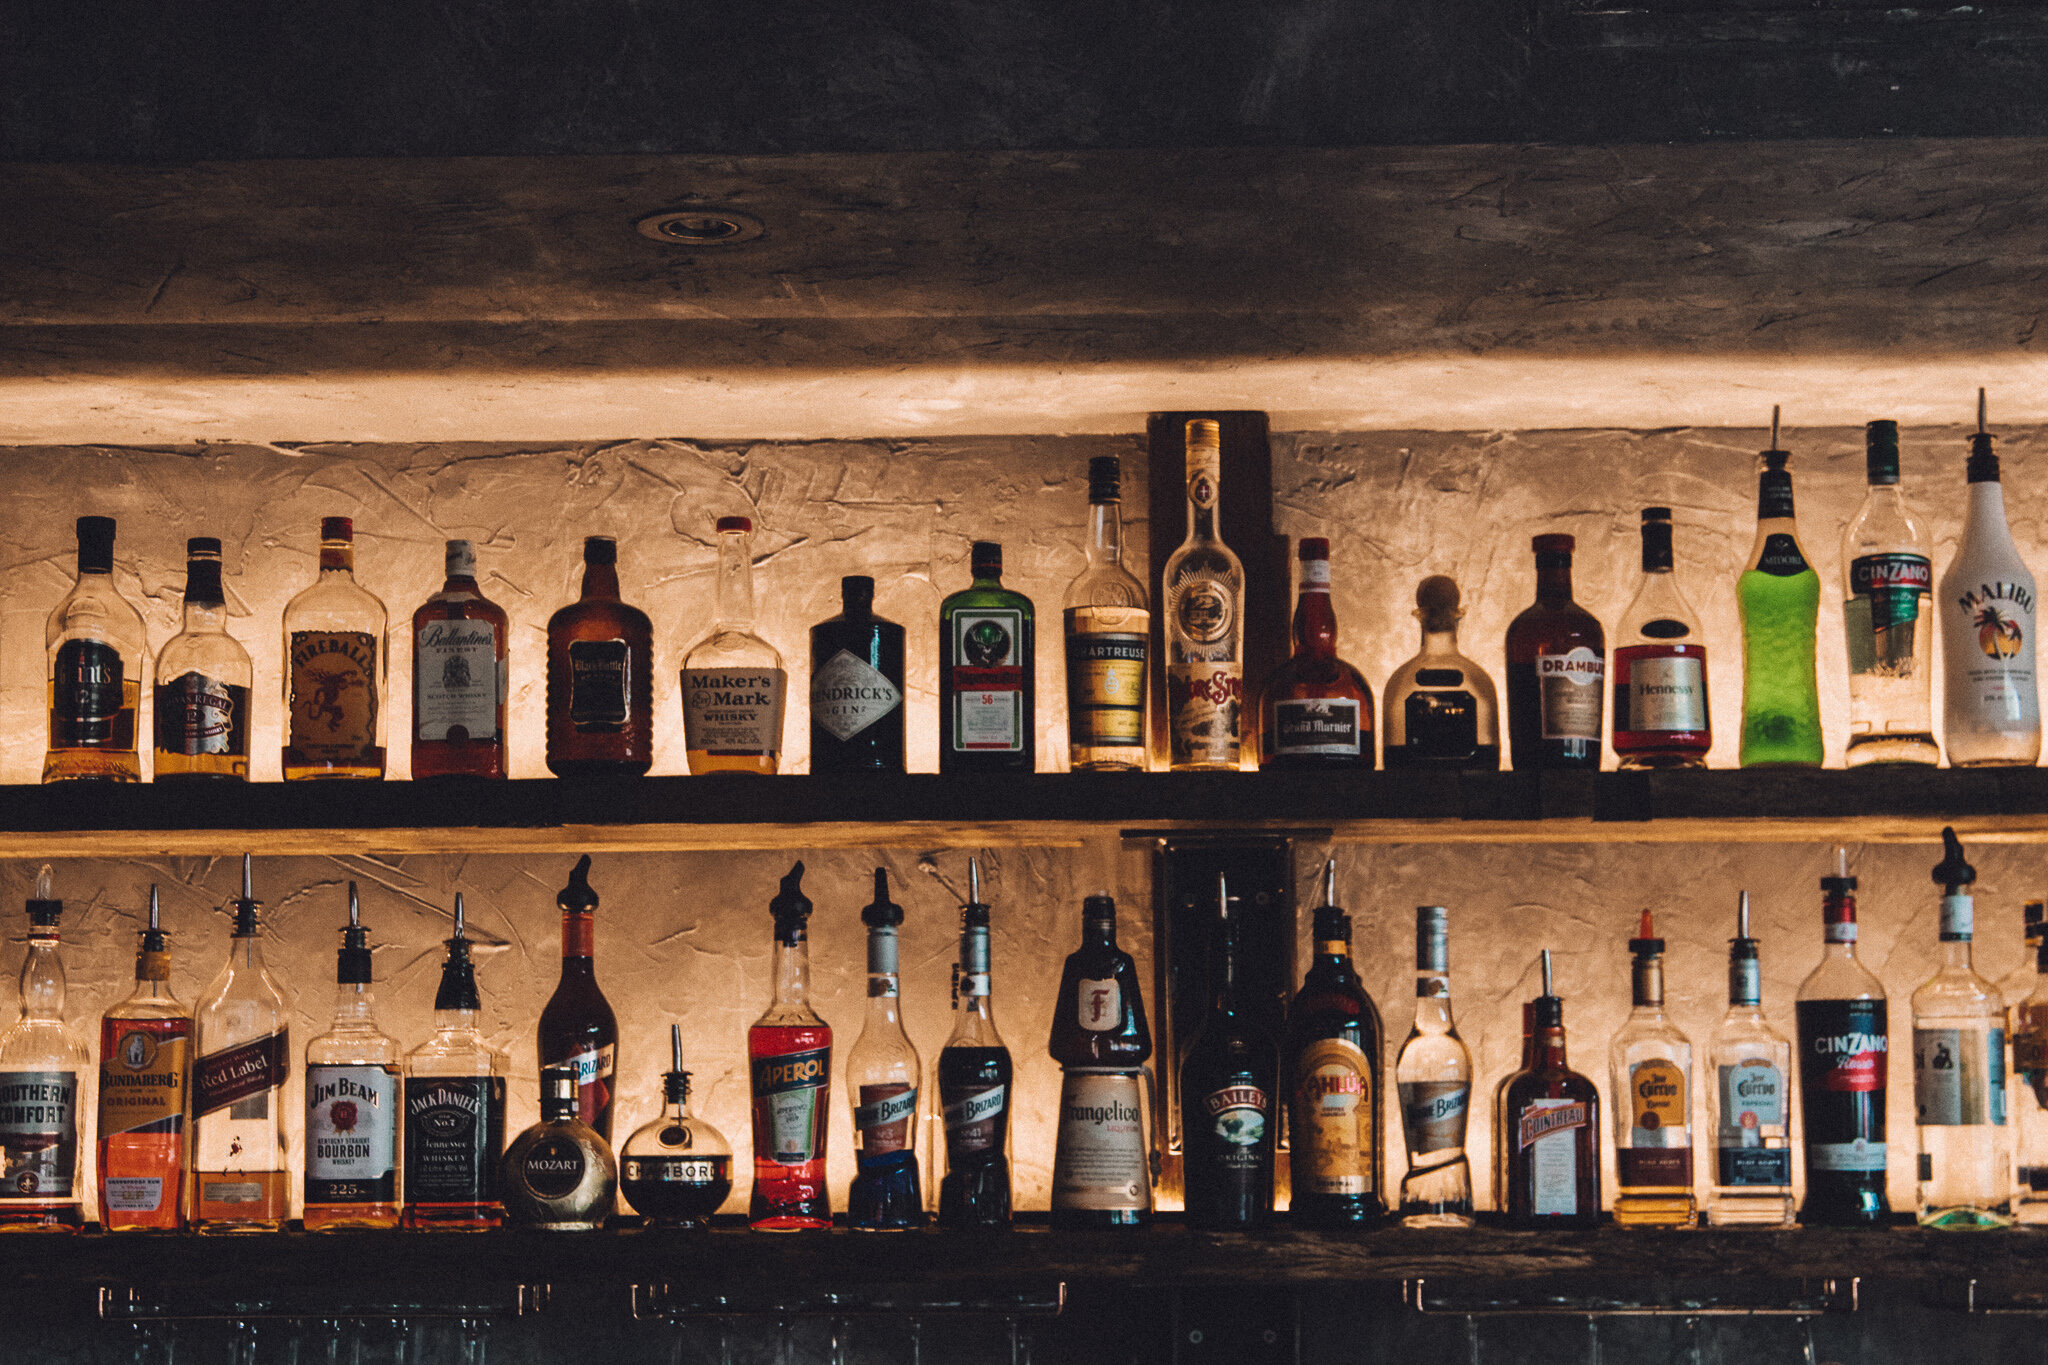
\includegraphics[width=2cm]{5.png}
    \end{multicols}

    Thus by considering the family supersets of the arbitrary element $a$, we see that the necessary and sufficient condition holds and therefore \textbf{Alfresco Italian Restaurant} is at least one of the best places to eat and drink in the Surfer's Paradise.
\end{Proof}







\end{document}
